%----------------------------------------------------------
% PACKAGES AND THEMES
%----------------------------------------------------------
\documentclass[aspectratio=169,xcolor=dvipsnames,handout]{beamer}

\usetheme{Darmstadt}
\usecolortheme{seahorse}
\setbeamercovered{transparent}

%\usepackage[hangul]{kotex}
\usepackage{hyperref}
\usepackage{graphicx, array, adjustbox, makecell}
\usepackage{booktabs, multicol, multirow}

% font조정
%\usepackage{fontspec}
%\setmainfont{Times New Roman}
%\setmainhangulfont{NanumGothic}

% 문자열 대체{노사관계론 전용}
\usepackage{newunicodechar}
\newunicodechar{•}{$\cdot$}
\newunicodechar{➔}{$\implies$}
\newunicodechar{∴}{$\therefore$}
\newunicodechar{∵}{$\because$}

%----------------------------------------------------------
% TITLE PAGE
%----------------------------------------------------------
\title{Can Mandatory Local-Talent Hiring Policy Reduce Regional Starting Wage Gap? Causal Evidence from Korean Graduates}
\subtitle{Oh \& Lee, 2024, \textit{Economic Analysis and Policy}, 84, 208–229}
\author[Oh \& Lee]{Sungjae Oh\inst{1} \and Hanol Lee\inst{2}}
\institute[CNU / SUFE]
{%
  \inst{1}
  %Department of Economics\\
  Chungnam National University, Korea\\
  \vspace{0.2cm}
  \inst{2}
  %Research Institute of Economics and Management\\
  Southwestern University of Finance and Economics, China\\
  \vspace{0.4cm}
  Presented at Korea Institute for Health and Social Affairs
}
\date[Nov, 2024]{\today}

%----------------------------------------------------------
\begin{document}
%----------------------------------------------------------

\frame{\titlepage}

\begin{frame}{Table of Contents}
    \small
    \tableofcontents[hideallsubsections]
\end{frame}

\section{Backgrounds}
\begin{frame}
    \frametitle{Regional disparities in Korea}
    \begin{itemize}[<+->]
        \item Severe disparities between capital area (Seoul Metropolitan Area, SMA) and the rest of the country
        \begin{itemize}[<+->]
            \item Concentration of economic, social, and educational resources in Seoul
            \item Seoul's GDP\@: 22.7\% of national total in 2022 (Statistics Korea, 2022).
            \item 9.8\% average wage gap between SMA and non-SMA workers in 2020 (Kang, 2023).
        \end{itemize}
        \item Significant educational gap
        \begin{itemize}[<+->]
            \item 14 out of Korea's top 20 universities located in Seoul (QS World University Rankings 2019)
            \item Labor market disadvantages for graduates from non-Seoul universities.
        \end{itemize}
    \end{itemize}
\end{frame}

\begin{frame}
    \frametitle{Mandatory local-talent hiring policy}
    \begin{itemize}[<+->]
        \item Innovation Cities Act implemented in 2007
        \begin{itemize}[<+->]
            \item The Act aims to decentralize the concentration of public institutions and corporations in the SMA and relocate them to designated innovation cities in non-SMA regions. 
        \end{itemize}
        \item Mandatory local-talent hiring policy introduced in 2013
        \begin{itemize}[<+->]
            \item In 2013, the Act mandates the recruitment of local talent, stipulating that relocated public sectors should hire a defined percentage of local talent, offering competitive wages with guaranteed tenure (Kim, 2019). 
        \end{itemize}
        \item ``Local talent''
        \begin{itemize}[<+->]
            \item Refers to graduates (or prospective graduates) of universities located in 14 non-SMA regions.
            \item Talent is recognized as local only in the region where their university campus is located. 
        \end{itemize}
    \end{itemize}
\end{frame}

\begin{frame}[allowframebreaks]
    \frametitle{Cumulative public sectors mandated to hire local talent since 2013}
    \begin{itemize}[<+->]
        \item 128 public sectors required to hire local talent by 2020
        \item Local talent hiring increased from 2.8\% (2012) to 14.2\% (2017)
        \item Projected to reach 30\% by 2022
        \item Three types of changes
        \begin{enumerate}
            \item Relocation of institutions: 2013--2015.
            \item Regional integration: Daegu-Gyeongbuk in 2016 and Chungnam-Chungbuk-Daejeon-Sejong in 2019.
            \item New designation: Chungnam, Chungbuk, Daejeon and Sejong in 2019.
        \end{enumerate}
    \end{itemize}
    \begin{table}[ht]
        \centering
        \scriptsize
        \begin{tabular}{lccccccccc}
        \toprule
        & \multicolumn{8}{c}{\textbf{Year}} \\
        \cline{2-9} 
        \textbf{Region} & 2013 & 2014 & 2015 & 2016 & 2017 & 2018 & 2019 & 2020 \\
        \midrule
        Busan     & 3 & 9  & 10 & 10 & 11 & 11 & 11 & 12 \\
        Ulsan     & 0 & 6  & 6  & 6  & 6  & 6  & 7  & 7  \\
        Gyeongnam & 0 & 3  & 7  & 9  & 10 & 10 & 10 & 10 \\
        Daegu     & 2 & 7  & 9  & 16 & 16 & 16 & 16 & 16 \\
        Gyeongbuk & 1 & 4  & 5  & 16 & 16 & 16 & 16 & 16 \\
        Jeonbuk   & 1 & 2  & 4  & 5  & 6  & 6  & 6  & 6  \\
        Gwangju   & 0 & 10 & 11 & 11 & 12 & 12 & 13 & 13 \\
        Jeonnam   & 0 & 10 & 11 & 11 & 12 & 12 & 13 & 13 \\
        Daejeon   & 0 & 0  & 0  & 0  & 0  & 0  & 0  & 51 \\
        Chungbuk  & 3 & 6  & 7  & 7  & 8  & 9  & 10 & 51 \\
        Chungnam  & 0 & 0  & 2  & 2  & 2  & 2  & 2  & 51 \\
        Sejong    & 1 & 14 & 18 & 18 & 19 & 19 & 19 & 51 \\
        Gangwon   & 1 & 4  & 8  & 9  & 10 & 10 & 10 & 10 \\
        Jeju      & 0 & 0  & 1  & 1  & 1  & 3  & 3  & 3  \\
        \bottomrule
        \end{tabular}
        \caption{Number of Firms Affected by the Policy by Year and Region}
    \end{table}
\end{frame}

\section{Main Objective}
\begin{frame}
    \frametitle{Research objectives}
    \begin{itemize}[<+->]
        \item Analyze wage gap between graduates from non-SMA universities and Seoul-based universities
        \item Investigate the impact of mandatory local-talent hiring policy on regional wage disparities
    \end{itemize}
\end{frame}

\begin{frame}
    \frametitle{Key findings}
    \begin{itemize}[<+->]
        \item Substantial regional wage disparities: Non-Seoul university graduates earn 10.9% less than Seoul graduates
        \item Policy effectively narrows wage gap between non-SMA and Seoul-based university graduates
        \item Stronger treatment effect for humanities graduates compared to science majors 
        \begin{itemize}[<+->]
            \item Possibly due to job characteristics of relocated public sectors
        \end{itemize}
        \item Policy incentivizes non-SMA universities to enhance educational quality Contributes to reduction in wage disparity
    \end{itemize}
\end{frame}

\begin{frame}
    \frametitle{Contributions to the literature}
    \begin{enumerate}[<+->]
        \item First study to measure policy impacts on labor market outcomes using micro-level data
        \item Estimates wage gap for early-career graduates by university category
        \begin{itemize}[<+->]
            \item Mitigates bias from accumulated work experience
            \item Focuses on the most affected group
        \end{itemize}
        \item Uncovers underlying policy mechanism
        \begin{itemize}[<+->]
            \item Policy incentivized non-SMA universities to enhance educational offerings
        \end{itemize}
    \end{enumerate}
\end{frame}

\section{Data and Model}%

\begin{frame}
    \frametitle{Data}
    \begin{itemize}[<+->]
        \item Data source: Graduates Occupational Mobility Survey (GOMS) 2010--2019.
        \begin{itemize}
            \item A repeated cross-sectional dataset.
        \end{itemize}
        \item The survey respondents complete the survey 12 to 18 months after their college graduation
        \item Sample: paid workers who graduated from 4-year universities
        \begin{itemize}
            \item Excluded: Medical/dental graduates, transfer students, pre-2009 graduates, those working abroad, military non-compliants males, and individuals aged 35+
        \end{itemize}
    \end{itemize}
\end{frame}

\begin{frame}[allowframebreaks]
    \frametitle{Methodology}
    \begin{enumerate}[<+->]
        \item Examine regional wage disparities based on the location of the universities.
        \begin{equation}
        \ln{(\text{wage})}_{i,j,p,t} = \alpha + \beta_1 \text{NonSeoul}_j + X_{i,t} \gamma + \tau_t + \epsilon_{i,j,p,t}
        \end{equation}
        \begin{itemize}[<+->]
            \item $\ln{(\text{wage})}_{i,j,p,t}$: The logarithm of monthly wages of individual i who graduated from university j located in region p in year t.
            \item $\text{NonSeoul}_j$: A dummy variable whether university j is located in outside of Seoul.
            \item $X_{i,t}$: Controls include age, age squared, work experience, work experience squared, gender, major, whether they attended the main campus, the percentile group to which a respondent's GPA belongs within their school's GPA distribution, and whether they graduated from elite high schools. 
        \end{itemize}
    \framebreak%
        \item Investigate the wage disparities between different types of non-SMA universities and Seoul-based universities. 
        \begin{equation}
            \ln{(\text{wage})}_{i,j,p,t} = \alpha + \beta_8 \text{NonSMA}_j + X_{i,t} \gamma + \theta_p + \tau_t + \epsilon_{i,j,p,t}
        \end{equation}
        \begin{equation}
            \ln{\text{wage}}_{i,j,p,t} = \alpha + \beta_9 \text{KNU9}_j + \beta_{10} \text{PubUj}_j + \beta_{11} \text{PriUj}_j + X_{i,t} \gamma + \theta_p + \tau_t + \epsilon_{i,j,p,t}
        \end{equation}
        \begin{itemize}[<+->]
            \item Benchmark group: Two ranking categories for baseline universities in Seoul: 1--20 and 21--50.
            \item KNU9 ($\text{KNU9}_j$), non-SMA public universities ($\text{PubUj}_j$), and non-SMA private universities ($\text{PriUj}_j$) to estimate the wage gap for each category of non-SMA universities relative to Seoul-based universities. 
        \end{itemize}
    \framebreak%
        \item Estimate the impact of the policy on the wage gap between two groups, using DID.% 
            \begin{align}
                \ln{\text{wage}}_{i,j,p,t} &= \alpha + \delta_1 D_{p,t} \text{nonSMA}_j + \beta_8 \text{nonSMA}_j + D_{p,t} \\ \nonumber
                    &\quad + X_{i,t} \gamma + \theta_p + \tau_t + \epsilon_{i,j,p,t} \\
                \ln{\text{wage}}_{i,j,p,t} &= \alpha + \delta_2 D_{p,t} \text{KNU9}_j + \delta_3 D_{p,t} \text{PubUj} 
                    + \delta_4 D_{p,t} \text{PriUj} + \beta_9 \text{KNU9}_j \\
                    &\quad + X_{i,t} \gamma + \theta_p + \tau_t + \epsilon_{i,j,p,t} \nonumber
            \end{align}
            \begin{itemize}[<+->]
                \item Control group: Two ranking categories for baseline universities in Seoul: 1--20 and 21--50.
                \item $D_{p,t}$: A dummy variable indicates whether the policy was implemented in region p in year t. Both dummy and continuous treatment variables to account for the scale of policy benefits.
            \end{itemize}
    \end{enumerate}
\end{frame}

\begin{frame}
    \frametitle{Summary statistics}
    \begin{itemize}[<+->]
        \item The outcome variable is the logarithm of monthly wages, measured in 2010 Korean Won. The mean log monthly wage is approximately 5.2, equivalent to 1.97 million Korean Won (or 1,704 US Dollars), based on 2010 prices. 
    \end{itemize}
    \begin{table}[ht]
        \tiny
        \centering
        \begin{tabular}{lcccc}
        \toprule
        \textbf{Variables} & \textbf{Mean} & \textbf{Std. Dev.} & \textbf{Min} & \textbf{Max} \\
        \midrule
        Log (monthly wage, 2010 Korean Won) & 5.188 & 0.453 & 3.117 & 6.244 \\
        Continuous treatment variable (No.\ of firms affected by the policy at province \(p\) and year \(t\)) & 3.816 & 5.243 & 0 & 19 \\
        Non-SMA universities          & 0.750 & 0.433 & 0 & 1 \\
        Non-SMA national universities & 0.172 & 0.377 & 0 & 1 \\
        Non-SMA public universities   & 0.108 & 0.310 & 0 & 1 \\
        Non-SMA private universities  & 0.470 & 0.499 & 0 & 1 \\
        \bottomrule
        \end{tabular}
    \end{table}
\end{frame}

\section{Main Results}%
\begin{frame}
    \frametitle{Regional disparities in graduates' wages}
    \begin{table}[ht]
        \centering
        \small
        \begin{tabular}{lc}
        \toprule
        \textbf{Outcome}             & \textbf{(1)} \\
        \midrule
        Non-Seoul                    & -0.109***    \\
                                     & (0.007)      \\
        \midrule
        Observations                 & 79,899       \\
        R-squared                    & 0.156        \\
        Controls                     & Yes          \\
        Location of the workplace FE & Yes          \\
        Graduation year FE           & Yes          \\
        Survey year FE               & Yes          \\
        \bottomrule
        \multicolumn{2}{p{6cm}}{\tiny\textit{Notes:} The dependent variable is the logarithm of monthly real wages of university graduates\@. Robust standard errors are indicated in parentheses. *** indicates statistical significance at 1\%, ** at 5\%, and * at 10\%.} \\
        \end{tabular}
    \end{table}
\end{frame}

\begin{frame}
    \frametitle{Wage disparities between graduates from non-SMA universities and Seoul-based universities}
    \begin{table}[ht]
        \centering
        \tiny
        \begin{tabular}{lcccc}
        \toprule
                                                   & \textbf{(1)} & \textbf{(2)} & \textbf{(3)} & \textbf{(4)} \\
        \midrule
        \textbf{Outcome}                           & \multicolumn{4}{c}{\textbf{Log of monthly real wages}} \\
        \midrule
         Ranking of baseline universities in Seoul & 1--20     & 21--50    & 1--20     & 21--50    \\
        \midrule
        Non-SMA universities                       & -0.160*** & -0.102*** &           &           \\
                                                   & (0.009)   & (0.010)   &           &           \\
        KNU9                                       &           &           & -0.117*** & -0.058*** \\
                                                   &           &           & (0.011)   & (0.012)   \\
        Non-SMA public universities                &           &           & -0.149*** & -0.092*** \\
                                                   &           &           & (0.010)   & (0.011)   \\
        Non-SMA private universities               &           &           & -0.178*** & -0.119*** \\
                                                   &           &           & (0.009)   & (0.010)   \\
        \midrule                                    
        Observations                               & 57,909    & 49,743    & 57,909    & 49,743    \\
        R-squared                                  & 0.167     & 0.153     & 0.167     & 0.153     \\
        Controls                                   & Yes       & Yes       & Yes       & Yes       \\
        FEs                                        & Yes       & Yes       & Yes       & Yes       \\
        \bottomrule
        \multicolumn{5}{p{9cm}}{\tiny\textit{Notes:} The dependent variable is the logarithm of monthly real wages of university graduates\@. Robust standard errors are indicated in parentheses. *** indicates statistical significance at 1\%, ** at 5\%, and * at 10\%.} \\
        \end{tabular}
    \end{table}
\end{frame}

\begin{frame}
    \frametitle{Impacts of the policy on the log of monthly real wages }
    \begin{table}[ht]
        \scriptsize
        \centering
        \begin{tabular}{lcc}
        \toprule
        & \textbf{(1)} & \textbf{(2)} \\
        \midrule
        \textbf{Outcome} & \multicolumn{2}{c}{\textbf{Log of monthly real wages}} \\
        \midrule
        Ranking of baseline universities in Seoul & 1--20     & 21--50  \\
        \midrule                                                                                  
        Non-SMA universities $\times D_{pt}$      & 0.003***  & 0.002**   \\
                                                  & (0.001)   & (0.001)   \\
        Non-SMA universities                      & -0.172*** & -0.110*** \\
                                                  & (0.009)   & (0.010)   \\
        \midrule                                                          
        Observations                              & 57,746    & 49,580    \\
        R-squared                                 & 0.165     & 0.151     \\
        Controls                                  & Yes       & Yes       \\
        FEs                                       & Yes       & Yes       \\
        \bottomrule
        \multicolumn{3}{p{9cm}}{\tiny\textit{Notes:} The dependent variable is the logarithm of monthly real wages of university graduates\@. Robust standard errors are indicated in parentheses. *** indicates statistical significance at 1\%, ** at 5\%, and * at 10\%.} \\
        \end{tabular}
    \end{table}
\end{frame}

\begin{frame}
    \frametitle{Impacts of the policy on the log of monthly real wages by types of Non-SMA Univ.}
    \begin{table}[ht]
        \tiny
        \centering
        \begin{tabular}{lcc}
        \toprule
        & \textbf{(1)} & \textbf{(2)} \\
        \midrule
        \textbf{Outcome} & \multicolumn{2}{c}{\textbf{Log of monthly real wages}} \\
        \midrule
        Ranking of baseline universities in Seoul    & 1--20     & 21--50    \\
        \midrule                                                             
        KNU9 $\times D_{pt}$                         & 0.003***  & 0.003*    \\
                                                     & (0.001)   & (0.001)   \\
        Non-SMA public universities $\times D_{pt}$  & 0.003***  & 0.003**   \\
                                                     & (0.001)   & (0.001)   \\
        Non-SMA private universities $\times D_{pt}$ & 0.002***  & 0.001**   \\
                                                     & (0.001)   & (0.001)   \\
        KNU9                                         & -0.134*** & -0.071*** \\
                                                     & (0.014)   & (0.014)   \\
        Non-SMA public universities                  & -0.164*** & -0.104*** \\
                                                     & (0.012)   & (0.013)   \\
        Non-SMA private universities                 & -0.185*** & -0.124*** \\
                                                     & (0.009)   & (0.010)   \\
        \midrule                                                             
        Observations                                 & 57,909    & 49,743    \\
        R-squared                                    & 0.169     & 0.125     \\
        Controls                                     & Yes       & Yes       \\
        FEs                                          & Yes       & Yes       \\
        \bottomrule
        \end{tabular}
    \end{table}
\end{frame}

\begin{frame}
    \frametitle{Impacts of the policy on the log of monthly real wages by major}
    \begin{table}[ht]
        \tiny
        \centering
        \begin{tabular}{lcccccc}
        \toprule
        & \textbf{(1)} & \textbf{(2)} & \textbf{(3)} & \textbf{(4)} \\
        \midrule
        \textbf{Outcome} & \multicolumn{4}{c}{\textbf{Log of monthly real wages}} \\
        \midrule
        \textbf{Major} & \multicolumn{2}{c}{\textbf{Humanities}}& \multicolumn{2}{c}{\textbf{Science}} \\
        \midrule                                                                                  
        Ranking of baseline universities in Seoul    & 1--20     & 21--50    & 1--20     & 21--50    \\
        \midrule                                                          
        KNU9 $\times D_{pt}$                         & 0.004***  & 0.003*    & 0.004***  & 0.003**** \\
                                                     & (0.002)   & (0.002)   & (0.001)   & (0.001)   \\
        Non-SMA public universities $\times D_{pt}$  & 0.005***  & 0.004**   & 0.002*    & 0.002     \\
                                                     & (0.002)   & (0.002)   & (0.001)   & (0.001)   \\
        Non-SMA private universities $\times D_{pt}$ & 0.003***  & 0.002**   & 0.002**   & 0.002**   \\
                                                     & (0.001)   & (0.001)   & (0.001)   & (0.001)   \\
        KNU9                                         & -0.168*** & -0.050*** & -0.119*** & -0.111*** \\
                                                     & (0.013)   & (0.016)   & (0.012)   & (0.014)   \\
        Non-SMA public universities                  & -0.199*** & -0.084*** & -0.149*** & -0.141*** \\
                                                     & (0.015)   & (0.018)   & (0.012)   & (0.014)   \\
        Non-SMA private universities                 & -0.238*** & -0.124*** & -0.155*** & -0.149*** \\
                                                     & (0.009)   & (0.013)   & (0.010)   & (0.012)   \\
        \midrule                                                          
        Observations                                 & 24,271    & 19,809    & 28,412    & 25,034    \\
        R-squared                                    & 0.169     & 0.125     & 0.169     & 0.125     \\
        Controls                                     & Yes       & Yes       & Yes       & Yes       \\
        FEs                                          & Yes       & Yes       & Yes       & Yes       \\
        \bottomrule
        \end{tabular}
    \end{table}
\end{frame}

\begin{frame}
    \frametitle{Results of Parallel Trend Test}
    \centering
    \begin{figure}
        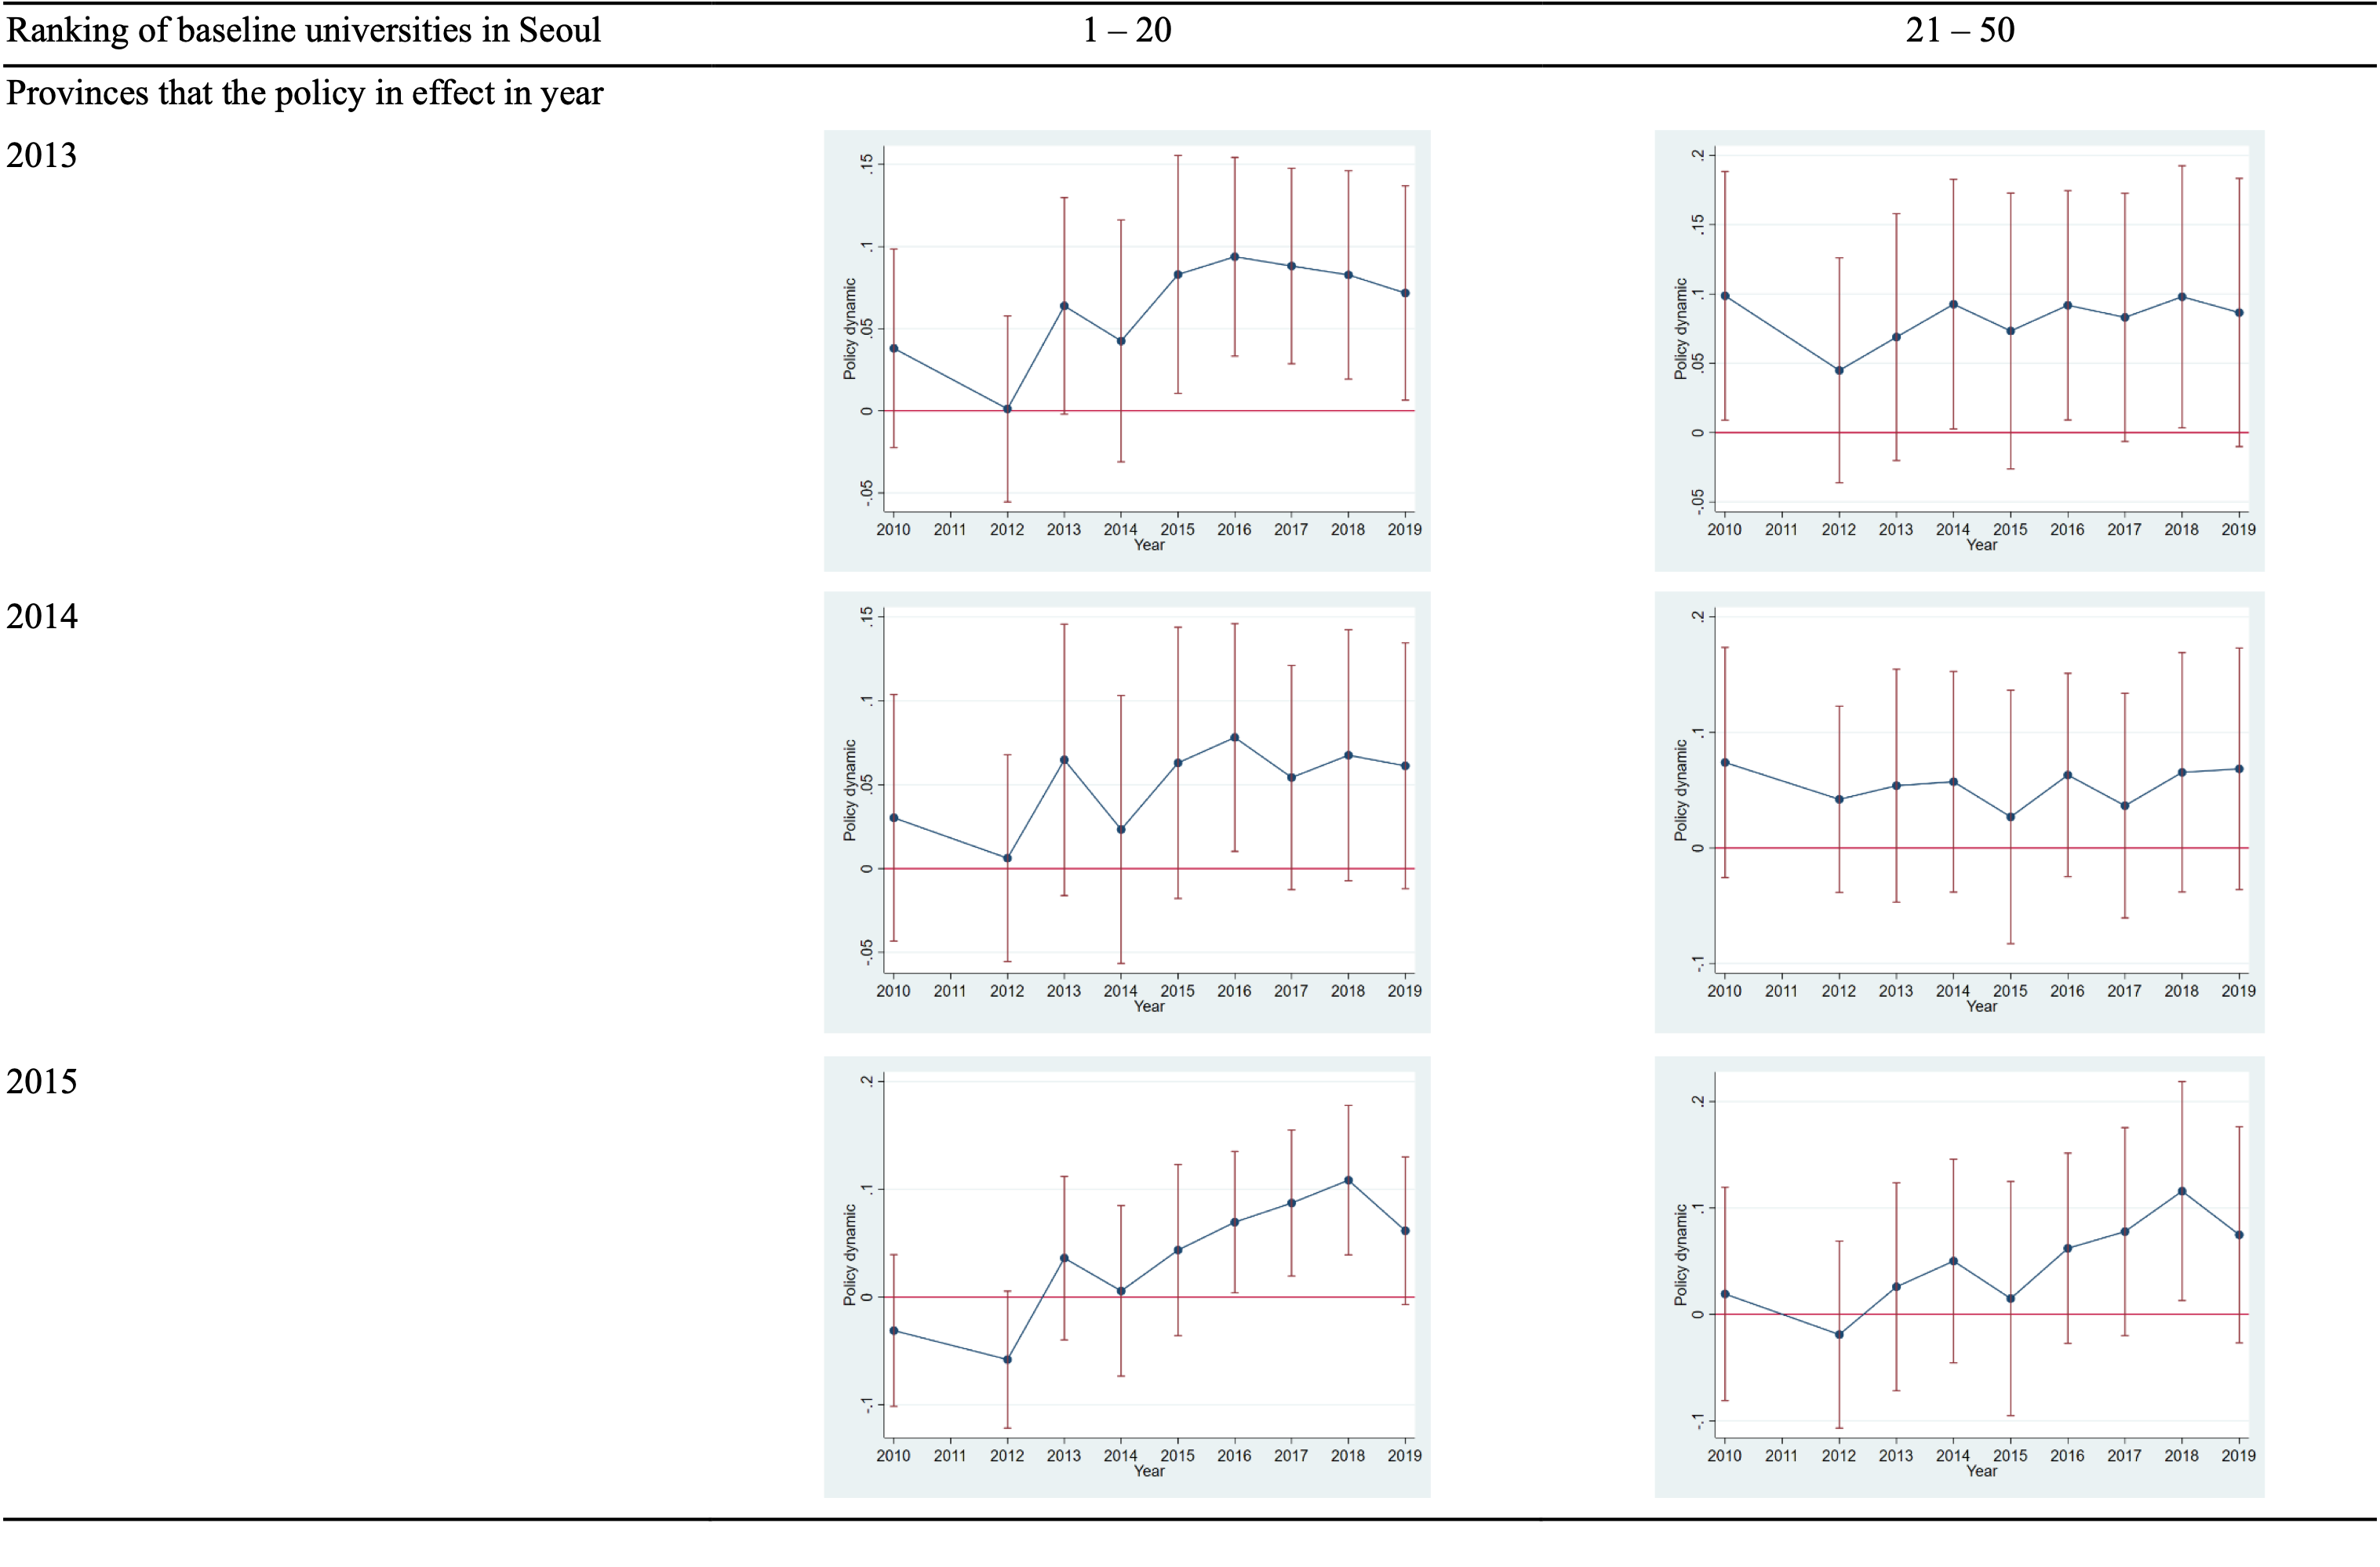
\includegraphics[width=.7\textwidth]{pic/pttest.png}
    \end{figure}
\end{frame}


\section{Mechanism}%
\begin{frame}[allowframebreaks]
    \frametitle{Mechanism test}
    Two potential mechanisms:
    \begin{enumerate}[<+->]
        \item Change in student enrollment behavior
        \begin{itemize}
            \item Potential shift from Seoul to non-SMA universities
            \item Could lead to higher-quality freshmen in non-SMA universities
            \item Study design mitigates this effect:
            \begin{itemize}
            \item Most of sample entered university before 2013
            \item Excludes policy effects through talent distribution changes
            \end{itemize}
        \end{itemize}
        \item Improvement in non-SMA university education quality
        \begin{itemize}
            \item Policy incentivizes enhancement of education quality
            \item Focus on job placement education
            \item Results in better labor market performance for graduates
        \end{itemize}
    \end{enumerate}
\end{frame}

\begin{frame}[allowframebreaks]
    \frametitle{Test results}
    \begin{table}
        \scriptsize
        \centering
        \begin{tabular}{lcc}
        \toprule
        & (1) & (2) \\
        \midrule
        \textbf{Outcome} & \multicolumn{2}{p{5cm}}{\textbf{JoongAng Ilbo University Rankings by year (between 2010 and 2019, times with minus 1)}} \\
        \midrule
        Ranking of baseline universities in Seoul & \multicolumn{2}{c}{1--20} \\
        \midrule
        KNU9 $\times$ Dpt & 0.239***   & 0.167***   \\
                        & (0.115)    & (0.100)    \\
        KNU9              & -13.359*** & -14.744*** \\
                        & (1.070)    & (1.173)    \\
        \midrule
        Observations      & 118        & 118        \\
        R-squared         & 0.647      & 0.785      \\
        Controls          & No         & Yes        \\
        Year FE           & Yes        & Yes        \\
        \bottomrule
        \multicolumn{3}{p{11cm}}{\tiny\textit{Notes:} The dependent variable is the annual university ranking\@. The controls include the number of faculty members, scholarships per enrolled student, the number of students in field practice, and the number of students involved in exchanges with foreign universities. Robust standard errors are indicated in parentheses. *** indicates statistical significance at 1\%, ** at 5\%, and * at 10\%.} \\
        \end{tabular}
    \end{table}
    \framebreak%
    \begin{table}
        \scriptsize
        \centering
        \begin{tabular}{lcc}
        \toprule
        & (1) & (2) \\
        \midrule
        \textbf{Outcome} & \multicolumn{2}{p{5cm}}{\textbf{Annual university-level GPA (max = 100, min = 0)}} \\
        \midrule
        Ranking of baseline universities in Seoul & \multicolumn{2}{c}{1--20} \\
        \midrule
        Non-SMA universities $\times$ Dpt         & 0.065*** & 0.081*** \\
                                                & (0.025)  & (0.023)  \\
        Non-SMA universities                      & 1.207*   & -0.029   \\
                                                & (0.674)  & (0.828)  \\
        \midrule
        Observations                              & 1,678    & 1,678    \\
        R-squared                                 & 0.037    & 0.064    \\
        Controls                                  & No       & Yes      \\
        Year FE                                   & Yes      & Yes      \\
        \bottomrule
        \multicolumn{3}{p{11cm}}{\tiny\textit{Notes:} The dependent variable is the annual university-level GPA\@. The controls include the number of faculty members, scholarships per enrolled student, the number of students in field practice, and the number of students involved in exchanges with foreign universities. Robust standard errors are indicated in parentheses. *** indicates statistical significance at 1\%, ** at 5\%, and * at 10\%.} \\
        \end{tabular}
    \end{table}
\end{frame}

\section{Concluding remarks}%

\begin{frame}
    \frametitle{Concluding remarks}
    \begin{itemize}[<+->]
        \item Mandatory local-talent hiring policy contributes to reducing regional wage disparities.
        \item Improvement in educational quality of non-SMA universities.
        \item Policy shows promise in promoting balanced regional development.
        \item Focus on public sectors
        \begin{itemize}
            \item Simulation studies in Korea suggest that the impact of relocating prominent private enterprises outweighs that of any other policy (Jun, 2007). 
        \end{itemize}
        \item Geographical restrictions in talent recruitment.
        \begin{itemize}
            \item Expanding the geographical scope of talent recruitment, allowing cross-regional applications and hiring, even from different zones, could enhance policy effectiveness.
        \end{itemize}
    \end{itemize}
\end{frame}

\begin{frame}
    \centering
    \huge
    Thank you
\end{frame}


%------------------------------------------------
\end{document}
%------------------------------------------------
